\documentclass[11pt,a4paper]{scrartcl}

% allow footnotes inside a table.
\usepackage{footnote}
\makesavenoteenv{tabular}
\makesavenoteenv{table}

% Support for UTF-8 and non-English letters require the following two
\usepackage[T1]{fontenc}
\usepackage[utf8]{inputenc}
\usepackage[ruled]{algorithm2e}
\usepackage{fancyvrb}
% Font packages
\usepackage[default,defaultsans,oldstyle,proportional]{lato}
\usepackage[scaled]{beramono}
\usepackage{sfmath}
% Optimized justification via improved microtypography on character level
\usepackage{microtype}
\usepackage{ragged2e}
\usepackage[none]{hyphenat} % disable all hyphenation
\setlength{\emergencystretch}{3em} % allow extra hfill, needed if hyphenation disabled
%\overfullrule=1mm % mark overfull boxes
%\usepackage{showframe} % show edges of text areas
% Page layout
\usepackage[left=15mm,right=15mm,top=15mm,bottom=20mm,
   nohead,foot=10mm]{geometry}
% Page headers

\usepackage{xcolor} % to access the named colour LightGray
\definecolor{LightGray}{gray}{0.95}

\usepackage{minted}
\usepackage{scrlayer-scrpage}
\usepackage{lastpage}
% Page header
\KOMAoptions{headsepline=0pt,plainheadsepline=off}
\ihead*{}
\chead*{}
\ohead*{}
% Page footer
\KOMAoptions{footsepline=0pt,plainfootsepline=off}
\ifoot*{}
\cfoot*{Page \thepage{} of \pageref*{LastPage}}
\ofoot*{}
% Text layout
\KOMAoption{parskip}{never}
\newlength{\myparindent}
\newlength{\myparskip}
\setlength{\myparindent}{0pt}
\setlength{\myparskip}{5pt plus 1pt}
\setparsizes{\myparindent}{\myparskip}{0.1\linewidth plus 1fil}
\RedeclareSectionCommand[beforeskip=6pt,afterskip=3pt,afterindent=false]{section}
\RedeclareSectionCommand[beforeskip=6pt,afterskip=-0.5em,afterindent=false]{paragraph}
\RaggedRight

% Graphics
\usepackage{graphicx}
% Colour definitions
\usepackage{xcolor}
\definecolor{secondary}{HTML}{435584}
% Floats
\usepackage{subcaption}
% Listings
\usepackage{listings}
\lstset{language=C, basicstyle=\small\ttfamily,
   aboveskip=0pt, belowskip=0pt}
\usepackage{upquote} % to use correct glyphs for single-quote in verbatim
% SI units
\usepackage{siunitx}
\sisetup{per-mode = symbol, detect-all = true}
% Hyperlinks
\usepackage[
   colorlinks=true,allcolors=secondary,breaklinks=true,
   bookmarks=true,unicode=true,bookmarksopen,bookmarksnumbered]{hyperref}
\usepackage{multicol}
% Package for inline, verbatim text (code snippets)
\usepackage{fancyvrb}
% Math environments, including align(*)
\usepackage{amsmath, amsfonts, amsthm, amssymb}
\usepackage{mathtools, nccmath}
\usepackage{physics}

% change figure placement
\usepackage{float}

% define a new float environment called a Listing, for code snippets.
\newfloat{lstfloat}{htbp}{lop}
\floatname{lstfloat}{Listing}
\def\lstfloatautorefname{Listing} % needed for hyperref/auroref

% define a critical section block
\SetKwBlock{CritSection}{critical section}{}

\hypersetup{
   colorlinks   = true
}

\newtheorem{theorem}{Theorem}[section]
\newtheorem{corollary}{Corollary}[theorem]
\newtheorem{lemma}[theorem]{Lemma}
\newtheorem{definition}[theorem]{Definition}
\newtheorem{proposition}[theorem]{Proposition}
\newtheorem{example}[theorem]{Example}

\usepackage{tikz}
\usetikzlibrary{automata, positioning}
\tikzset{->, node distance=3cm}

\title{The PixARLang compiler}
\subtitle{CPS2000 Compiler Theory and Practice}
\author{Mark Mizzi}
\date{Last edited: \today}

% \verb in a footnote
\VerbatimFootnotes

\begin{document}

\maketitle

\tableofcontents

\newpage

\section{Introduction}

This report describes the implementation of a compiler for the PixAR langauge targeting the PixAR virtual machine.

\subsubsection{Code standards and organization}

The code for the project is written using C++17, and makes use of several modern features in the language, including \href{https://en.cppreference.com/mwiki/index.php?title=cpp/language/structured_binding&oldid=150915}{structured binding}, and the \href{https://en.cppreference.com/mwiki/index.php?title=cpp/utility/variant&oldid=150622}{\verb|std::variant|} container.

The \href{https://cmake.org}{CMake} build system is used to manage and compile the source code. In order to build the project, run the following commands from the root directory:
\begin{minted}[bgColor=LightGray]{bash}
cmake -DCMAKE_EXPORT_COMPILE_COMMANDS=ON -DCMAKE_BUILD_TYPE=Release .
make
\end{minted}

The source code itself can be found in the \verb|src/| subdirectory, and is organized into files as shown in Figure~\ref{fig:code-organization}. There are also some example PixAR programs used to test the compiler in the \verb|examples/| subdirectory.

This report is written in Latex and its source can be found in the \verb|report/| subdirectory of the project. It can be compiled by running the following commands:
\begin{minted}[bgColor=LightGray]{bash}
cd report
make
\end{minted}

\subsubsection{Video presentation}

A video presentation of the compiler can be found at %% TODO

\newpage

\section{Lexing}

\subsection{Design considerations}

THere are several approaches available to the implementer when it comes to writing a hand-coded lexer.

The implementation uses a table-driven approach to lexing. This approach assumes that the micro-syntax of each token type $t_{i}$ can be specified using a regular expression $e_{i}$. The lexer emulates a particular DFSA (deterministic finite state automaton) that accepts the language specified by the following regular expression:
$$ e = e_{1} | ... | e_{k} $$

The DFSA emulated by this compiler's lexer is shown in Figure~\ref{fig:lexer-dfsa}.

\begin{figure}[H]
  \centering
  \caption{DFSA that lexes tokens in the PixAR language.}~\label{fig:lexer-dfsa}
\begin{tikzpicture}
\node[state] (a) { $START$ };
\node[state, accepting, right of=a] (id) { $ID$ };
\node[state, accepting, above of=a] (colon) { $COLON$ };
\node[state, accepting, above right of=a] (comma) { $COMMA$ };
\node[state, accepting, below right of=a] (greater) { $GREATER$ };
\node[state, accepting, below of=a] (less) { $LESS$ };
\node[state, accepting, below left of=a] (assign) { $ASSIGN$ };
\node[state, accepting, left of=a] (plus) { $PLUS$ };
\node[state, accepting, above left of=a] (minus) { $MINUS$ };
\node[state, accepting, left of=minus] (div) { $DIV$ };
\node[state, accepting, left of=plus] (star) { $STAR$ };
\node[state, accepting, below right of=greater] (ge) { $GE$ };
\node[state, accepting, below of=less] (le) { $LE$ };
\node[state, accepting, below left of=assign] (eq) { $EQ$ };
\node[state, accepting, above left of=minus] (arrow) { $ARROW$ };

\draw (a) edge[above] node{a-zA-Z\_} (id)
    (id) edge[loop right] node{a-zA-Z\_0-9} (id)
    (a) edge[left] node{:} (colon)
    (a) edge[above] node{,} (comma)
    (a) edge[above] node{>} (greater)
    (greater) edge[above] node{=} (ge)
    (less) edge[right] node{=} (le)
    (a) edge[right] node{<} (less)
    (a) edge[above] node{=} (assign)
    (assign) edge[above] node{=} (eq)
    (a) edge[above] node{+} (plus)
    (a) edge[bend left, below] node{*} (star)
    (a) edge[below] node{/} (div)
    (a) edge[above] node{-} (minus)
    (minus) edge[above] node{>} (arrow);

\end{tikzpicture}
\end{figure}

The transition table of the deterministic finite state automaton is stored in an auxiliary data structure, and a ``skeleton'' function uses this table to carry out lexing itself. Pseudo-code for this function is shown in Algorithm~\ref{lst:lexer}.

% \begin{algorithm}
% \caption{Pseudo-code for the ``skeleton'' function at the heart of the table-driven lexer}\label{lst:lexer}
% \begin{algorithmic}
%   \Require $n \geq 0$
%   \If{$Eof()$}
%     \State $\return Token(type=END)$
%   \EndIf

%   \While{$!Eof()$}

%   \EndWhile
% \State $c \gets nextChar()$
% \State $X \gets x$
% \State $N \gets n$
% \While{$N \neq 0$}
% \If{$N$ is even}
%     \State $X \gets X \times X$
%     \State $N \gets \frac{N}{2}$  \Comment{This is a comment}
% \ElsIf{$N$ is odd}
%     \State $y \gets y \times X$
%     \State $N \gets N - 1$
% \EndIf
% \EndWhile
% \end{algorithmic}
% \end{algorithm}

Several simplifying decisions were made in designing the lexer. Firstly, each valid input character was classified into a character class. The character classes are mutually exclusive, and group together characters which result in the same state transitions for each state of the DFSA. For example, the digit characters $0-9$ are classified into a single group. This greatly decreases the size of the table used. Choosing character classes is not as straightforward as it may seem, and new classes may be needed as more token types are added to the language. For example, although one may think it sufficient to create a single class for the alphabetic characters $a-zA-Z$, two classes are needed for $a-fA-F$ and $g-zG-Z$ as the former characters can appear in hexadecimal literals, whereas the latter cannot.

Secondly, a \verb!std::map! data structure was used to store the table. This allows us to encode the partial DFSA shown in Figure~\ref{fig:lexer-dfsa} directly. Transitions that would lead to an error state are ommitted from this map, and the skeleton function throws a \verb!LexerError! if it cannot make a transition while the current state is not an accepting state. The use of an array for storing the table would require transitions to an error state to be declared explicitly.

Finally, keywords are not handled directly by the table-driven portion of the lexer. Instead keywords are lexed as regular identifiers, and then filtered by another method which wraps the skeleton function. As a side effect of this design decision, the former function must also reject any identifiers which start with an underscore, which is disallowed by the language specification. This cannot be done by the skeleton function itself as certain keywords start with an underscore.

\subsection{Code organization}

\newpage

\section{Abstract Syntax tree, Visitors, and Parsing}

\subsection{Modifications made to eBNF}

% TODO

\subsection{Abstract syntax trees}

Abstract syntax trees are represented by an inheritance hierarchy shown in Figure~\ref{fig:ast-hierarchy}.

\begin{figure}
  \centering
  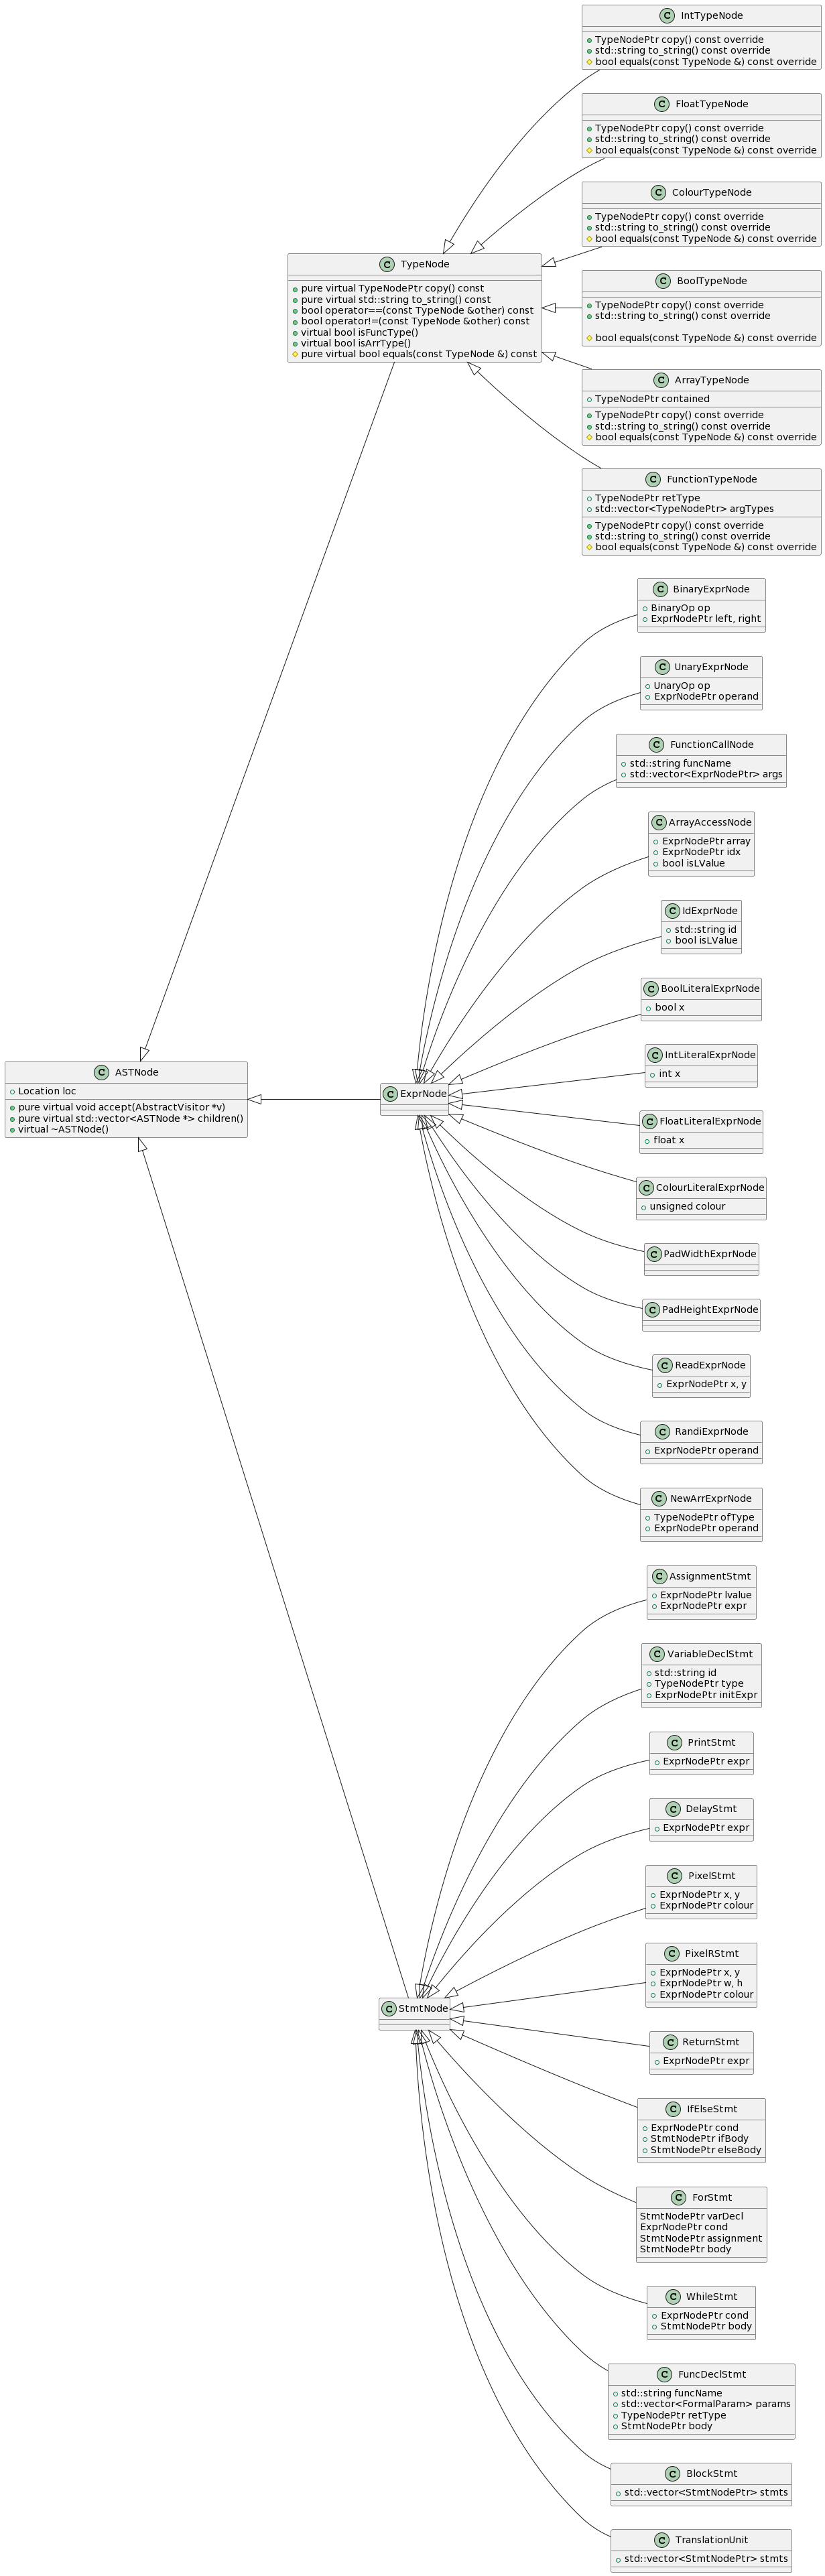
\includegraphics[height=0.95\textheight]{ast_uml}
  \caption{Inheritance hierarchy for AST nodes. Some methods are ommitted for brevity.}~\label{fig:ast-hierarchy}
\end{figure}

Every node type inherits from an \verb!ASTNode! abstract class. This class contains a \verb!Location! member that stores the position of the source code that produced the node. This allows the compiler to produce very useful error messages which indicate the location of the error to the user.

The \verb!ASTNode! type also contains a pure virtual method \verb!accept!, that subclasses must implement to support visitors. Another pure virtual method \verb!children! is implemented by subclasses to return their child nodes.

There are three direct subclasses of \verb!ASTNode!, which are themselves abstract: \verb!StmtNode!, \verb!ExprNode!, \verb!TypeNode!. These three subclasses represent the three basic kinds of syntactic structures in SIPLang: statements, expressions, and types.

Concrete subclasses of these three classes use \verb!unique_ptr! to reference child nodes.

Type nodes are used extensively in semantic checking. In order to aid this \verb!TypeNode! has additional methods \verb!copy! and \verb!to_string! which produces a deep copy of the node, and prints it in human readable form respectively.

Note that deep copying is necessary in the semantic checker due to the use of \verb!unique_ptr!. However, copying is rarely needed, and is considered a small cost compared to the convenience of using \verb!unique_ptr!.

In addition, type nodes also implement the comparision operator \verb!==!. Implementing comparision over a type hierarchy requires an unusual pattern. The implementation of \verb!operator==! in \verb!TypeNode! compares the \verb!typeid! of the two nodes being compared, and returns \verb!false! if they are not the same (dealing with the condition where the two \verb!TypeNode!s are of different types). Otherwise, a virtual \verb!equals! method is called.

In simple subclasses of \verb!TypeNode!, such as \verb!IntTypeNode! or \verb!FloatTypeNode!, this method simply returns true, as any two instances of such simple nodes are semantically equal.

For more complex subclasses, such as \verb!ArrayTypeNode!, the \verb!equals! method statically casts its argument to the type of the subclass. This is guaranteed to be type safe provided \verb!equals! is only called by \verb!operator==!. The \verb!equals! method can then perform subclass-specific equality checks, (in this case making sure the type of array elements is the same).

A subclass of \verb!TypeNode! called \verb!FunctionTypeNode! is used to represent function types during semantic checking. Nodes of this type are not produced during parsing, but are used to represent the type of function symbols.

Instances of \verb!TypeNode! also have \verb!isFuncType! and \verb!isArrType! methods which can be used to check whether a \verb!TypeNode! is an \verb!ArrayTypeNode! or a \verb!FunctionTypeNode! respectively.

\subsection{The Visitor Pattern}

The visitor pattern is widely used in compilers to cleanly separate an abstract syntax tree data structure from the implementation of algorithms that need to traverse it.

The SIPLang compiler employs a fairly pedestrian implementation of the visitor pattern. Visitors subclass an \verb!AbstractVisitor! class, which has an overloaded pure virtual \verb!visit! method for each concrete derived class of \verb!ASTNode!, which is passed as an argument (by reference):

\begin{minted}[bgColor=LightGray]{c++}
class AbstractVisitor {
public:
  virtual void visit(IntTypeNode &node) = 0;
  // ...
  virtual void visit(TranslationUnit &node) = 0;
\end{minted}

\verb!ASTNode! contains a pure virtual method called \verb!accept!, which takes a pointer to an \verb!AbstractVisitor! instance. Each concrete derived class of \verb!ASTNode! implements \verb!accept! to call the version of the \verb!visit! method that accepts its type:

\begin{minted}[bgColor=LightGray]{c++}
  void accept(AbstractVisitor *v) override { v->visit(*this); }
\end{minted}

In addition \verb!AbstractVisitor! has concrete methods \verb!visitChildren! and \verb!rvisitChildren!. These methods both take a pointer to an \verb!ASTNode! instance, and use its \verb!children! method to visit each of its child nodes (by calling the \verb!accept! method on each of the children). \verb!rvisitChildren! traverses the \verb!vector! of children in reverse order (this proves useful during code generation).

Concrete subclasses of \verb!AbstractVisitor! are used to generate XML for a parsed AST, for semantic checking, as well as for code generation.

\subsection{Design considerations for the parser}

The compiler uses a recursive descent parser which directly produces the AST.

Parse errors are handled by \verb!throw!ing an instance of \verb!ParserError!. This class inherits from the generic \verb!CompilationError! class, and reports an error message along with the location in the source file where the error originated.

Logic for the parser is encapsulated in a \verb!Parser! class. This class has two methods which are fundamental to parsing: \verb!peek! and \verb!consume!.

\verb!peek! takes an integer parameter \verb!i!, and looks ahead \verb!i! tokens in the token stream. Since tokens are obtained one by one from the lexer, and there is no way to look-ahead without consuming a token, the parser keeps an internal queue of tokens. If a lookahead smaller than the size of the queue is requested, \verb!peek! simply returns the appropriate token from the queue. Otherwise, the method gets the required tokens from the lexer and pushes them onto the queue, returning the last one.

Similarly \verb!consume! checks the internal queue. If it is non-empty, it pops and returns the token at the front of the queue. Otherwise, it gets the next token from the lexer, and returns it.

The parsing functions interact with the token stream through these functions. Due to the limited expressivity of SIPLang, the largest lookahead required is of 2 tokens. This lookahead of 2 tokens is used to differentiate between function calls (in which case a lookahead of 2 yields a \verb!(! token), or array accesses (in which case a lookahead of 2 yields a \verb![! token), or identity expressions.

In order to aid parsing, a \verb!CHECK_TOKEN! macro is used to check the type of a token with an expected type, and throw an appropriate \verb!ParserError! if the types don't match.

In general, duplicate or redundant checks are avoided in the parsing functions. For example, the method \verb!parseWhile! which parses a \verb!while! statement is only invoked by the \verb!parseStatement! function when the next lookahead token is a \verb!while! keyword token. The method therefore consumes a token without checking it, assuming that it is a \verb!while! keyword token.

In addition, recursion is avoided where possible. For example, where the EBNF of SIPLang specifies that zero or more repetitions of a non-terminal are part of a valid production rule, a loop is used to implement parsing of these repetitions. This makes construction of the AST simpler; nodes are simply accumulated into a vector, and then passed directly to the node constructor.

The following snippet shows the implementation of block parsing, which demonstrates the features described above:

\begin{minted}[bgColor=LightGray]{c++}
ast::StmtNodePtr Parser::parseBlock() {
  Location loc = consume().loc; // consume {

  std::vector<ast::StmtNodePtr> stmts;

  while (peek(0).type != lexer::RBRACE_TOK) {
    stmts.push_back(std::move(parseStatement()));
  }

  Location endloc = consume().loc; // consume }.

  return std::make_unique<ast::BlockStmt>(std::move(stmts), loc.merge(endloc));
}
\end{minted}

Firstly, note that the first token is consumed without checking that it is indeed a \verb!{! token. Its location is saved to a variable, as it is needed to construct the location of the node produced.

Secondly, note that statements are parsed using a \verb!while! loop, and collected in a \verb!vector!.

Finally, the \verb!}! token is consumed, and a new \verb!BlockStmt! node is constructed using the \verb!StmtNode!s parsed. There is no check to confirm that the last token consumed is a \verb!}! token, as this is the terminating condition of the \verb!while! loop.

\newpage

\section{XML generation}

XML generation is implemented using a subclass of \verb!AbstractVisitor! called \verb!XMLVisitor!.

Generating XML is straightforward, but tedious, so two macros, \verb!XML_ELEM_WITH_CHILDREN!, and \verb!XML_ELEM_WITH_CONTENT!, are used to ease the job. One of the macros generates XML for AST nodes which have children (using, among other things, the \verb!visitChildren! method), while the other generates XML for leaves of the AST tree, where the content between XML tags is derived directly from the node.

Each of these macros writes to a \verb!std::stringstream! in the \verb!XMLVisitor! class, which is used to store the incrementally generated XML. An \verb!indent! member variable is used to keep track of the current indentation level of the XML being produced.

The generated XML includes source locations for each of the AST nodes. In addition, special characters are sanitized. For example, the \verb!<! character is converted to \verb!&gt;!. This allows external programs, such as a browser, to correctly parse the XML produced.

Once an AST has been visited, the generated XML can be extracted from the visitor using the \verb!xml()! method, which simply produces a \verb!std::string! from the \verb!std::stringstream! member.

Listing~\ref{lst:example-xml-1} shows the XML generated by the compiler for the example program in Listing~\ref{lst:example-program-1}.

\begin{lstfloat}

\begin{minted}[bgcolor=LightGray]{text}
__pixelr 0, 0, 3, 4, #ff0000;
\end{minted}
  \caption{Example program which renders a red rectangle in the bottom left corner of the VM display}~\label{lst:example-program-1}
\end{lstfloat}

\begin{lstfloat}

\begin{minted}[bgcolor=LightGray]{xml}
<TranslationUnit loc="[1:0]-[1:29]">
 <PixelRStmt loc="[1:0]-[1:29]">
  <IntLiteralExprNode loc="[1:9]-[1:10]">0</IntLiteralExprNode>
  <IntLiteralExprNode loc="[1:12]-[1:13]">0</IntLiteralExprNode>
  <IntLiteralExprNode loc="[1:15]-[1:16]">3</IntLiteralExprNode>
  <IntLiteralExprNode loc="[1:18]-[1:19]">4</IntLiteralExprNode>
  <ColourLiteralExprNode loc="[1:21]-[1:28]">16711680</ColourLiteralExprNode>
 </PixelRStmt>
</TranslationUnit>
\end{minted}
  \caption{XML generated for the program shown in Listing~\ref{lst:example-program-1}}~\label{lst:example-xml-1}

\end{lstfloat}

\newpage

\section{Semantic checking}

\subsection{Types defined for semantic checking}

\subsubsection{Errors}

Semantic errors encountered while visiting an AST are handled by throwing an instance of \verb|SemanticError|, with a useful error message and the location of the error in the source code, which is obtained from the AST.

Semantic error subclasses \verb|CompilationError|, and simply calls its constructor with a formatted version of the error message passed to it, in similar fashion to \verb|LexerError| and \verb|ParserError|.

\subsubsection{Symbol tables}

The purpose of a symbol table is to map a \verb|StmtNode| in the AST to information about the symbols in the scope it defines. For example, a \verb|ForStmt| node gets mapped to a scope containing information about (at least) its loop variable. Not every type of \verb|StmtNode| can have a scope associated with it, for example \verb|AssignmentStmt| cannot.

Symbol tables are represented by a \Verb|SymbolTable| type. This is an alias for a \verb|std::map| which maps \verb|StmtNode| pointers to a \verb|Scope|.

\subsubsection{Scopes}~\label{scope-sect}

A \verb|Scope| is a struct which contains the actual symbol information inside a \verb|std::map| field that maps \verb|std::string| (identifiers) to a \verb|SymbolTableEntry| struct.

Aside from symbol information, \verb|Scope|s also contain a pointer to their parent scope (if any). This pointer is used in the \verb|get()| method of a \verb|Scope|, which returns the symbol information for a variable if it is in the current \verb|Scope| instance, or in some \verb|Scope| which can be reached via the parent pointer.

The \verb|get| method proves useful during semantic checking, chiefly when checking that a variable is defined at a point where it is referenced or assigned to.

\verb|Scope|s also contain a \verb|std::optional<FunctionTypeNode>| field, which contains nothing for most \verb|Scope|s, but contains the function type (signature) for the outermost scope of a function.

The \verb|getFuncType()| method gets the function type (signature) for the function which the scope is defined in. Since only the outermost scope of a function carries its signature, this method may recursively call itself on the parent scope.

\subsubsection{Symbol table entries}

\verb|SymbolTableEntry| instances hold the information for a specific program symbol. In the final compiler implemented, the only field in this struct is a \verb|std::unique_ptr<TypeNode>| field containing the type of the symbol. Types are deep copied from the AST when constructing a \verb|SymbolTableEntry|, using the \verb|copy()| method mentioned above.

Note that the semantic checker treats function names as regular symbols, and uses the same structures discussed above to keep track of information for them. This is catered to by the \verb|FunctionTypeNode| type, a subclass of \verb|TypeNode| which is not produced by a \verb|Parser|, but is used in \verb|SymbolTableEntry|.

\subsubsection{Type checking tables}

A \verb|TypeCheckerTable| is a temporary table used by the \verb|SemanticVisitor| class during semantic checking. It is a \verb|std::map| which maps \verb|ExprNode| pointers to a \verb|std::unique_ptr<TypeNode>|.

This allows an \verb|ExprNode| to be type checked by looking up the types of its subexpressions in an instance of \verb|TypeCheckerTable|.

\subsection{The semantic visitor}

Semantic checking is implemented using a subclass of \Verb|AbstractVisitor| called \Verb|SemanticVisitor|.

Information about program symbols is collected by the \Verb|SemanticVisitor|, and placed inside an instance of \Verb|SymbolTable|. This symbol table is also used by the code generation visitor, and hence a \Verb|SemanticVisitor| contains a reference to a \Verb|SymbolTable|, which is passed to it during construction (by an instance of the \verb|Compiler| class).

\verb|SemanticVisitor|s also contain a \verb|std::stack| of \verb|TypeCheckerTable|s. The visit methods for expression nodes first visit the child nodes (sub-expressions), and then type check the current node by looking up the type of the sub-expressions in the \verb|TypeCheckerTable| at the top of the stack.

Finally, provided that the type check succeeds, an entry mapping the current expression node to its type is placed in the \verb|TypeCheckerTable| at the top of the stack, so that it can be used to type-check parent nodes.

\verb|SemanticVisitor| also has a pair of \verb|enterScope|/\verb|exitScope| helper functions, which are used in \verb|visit| functions for \verb|StmtNode|s with an associated scope.

\verb|enterScope| adds a new entry to the \verb|SymbolTable| for the given \verb|StmtNode|, and sets the \verb|currentScope| pointer to point to the newly created \verb|Scope| instance (which has the old value of \verb|currentScope| as its parent). In addition, it pushes a new \verb|TypeCheckerTable| onto the stack.

\verb|exitScope| sets the \verb|currentScope| pointer to the old value's parent pointer, and pops a \verb|TypeCheckerTable| off the stack, effectively de-allocating it. This is a safe operation, as the types of sub-expressions within a scope cannot affect types of expressions in the parent scope.

This is precisely why a stack of \verb|TypeCheckerTable|s is used; the compiler saves memory by getting rid of type information when it is no longer needed.

Symbols can be accessed in a scope that is more deeply nested than the one in which they are defined; given this, one may ask how the stack of \verb|TypeCheckerTable|s can be used to get type information about symbols (since a \verb|TypeCheckerTable| has no parent pointer).

The answer lies in the implementation of the \verb|visit()| method for \verb|IdExprNode|. This method indiscrimately fetches type information for a symbol using the \verb|get()| method of \verb|currentScope|, and places it in the \verb|TypeCheckerTable| at the top of the stack, where it is available for type checking of parent expressions.

\subsubsection{Type checking}

Several checks were implemented in the \verb|SemanticVisitor|'s \verb|visit()| methods.

Firstly, as mentioned above, type checking was implemented for all compound expressions. Table~\ref{tab:type-checking-operators} shows valid type combinations for the binary and unary operators in the language. Table~\ref{tab:type-checking-builtins} shows the valid type combinations for builtin expressions and statements.

\begin{table}[ht]
  \centering
  \begin{tabular}{|c|c|c|c|}
    \hline
    Operator & Left operand type & Right operand type & Result type \\ \hline\hline
    \Verb|+|,\Verb|-|, \Verb|*| & \Verb|int| & \Verb|int| & \Verb|int|\\ \hline
    \Verb|+|,\Verb|-|, \Verb|*| & \Verb|float| & \Verb|float| & \Verb|float|\\ \hline
    \Verb|/| & \Verb|int| & \Verb|int| & \Verb|float| \\ \hline
    \Verb|/| & \Verb|float| & \Verb|float| & \Verb|float| \\ \hline
    \Verb|and|, \Verb|or| & \Verb|bool| & \Verb|bool| & \Verb|bool| \\ \hline
    \Verb|>|, \Verb|<|, \Verb|>=|, \Verb|<=| & \Verb|int| & \Verb|int| & \Verb|bool| \\ \hline
    \Verb|>|, \Verb|<|, \Verb|>=|, \Verb|<=| & \Verb|float| & \Verb|float| & \Verb|bool| \\ \hline
    \Verb|==|, \Verb|!=| & \Verb|int| & \Verb|int| & \Verb|bool| \\ \hline
    \Verb|==|, \Verb|!=| & \Verb|float| & \Verb|float| & \Verb|bool| \\ \hline
    \Verb|==|, \Verb|!=| & \Verb|bool| & \Verb|bool| & \Verb|bool| \\ \hline
    \Verb|==|, \Verb|!=| & \Verb|colour| & \Verb|colour| & \Verb|bool| \\ \hline
    \Verb|==|, \Verb|!=|\footnote{Array comparision is based on reference equality.} & \Verb|[]|$T$ & \Verb|[]|$T$ & \Verb|bool| \\ \hline
  \end{tabular}

  \begin{tabular}{|c|c|c|}
    \hline
    Operator & Operand & Result type \\ \hline\hline
    \Verb|!| & \Verb|bool| & \Verb|bool| \\ \hline
    \Verb|-| & \Verb|int| & \Verb|int| \\ \hline
    \Verb|-| & \Verb|float| & \Verb|float| \\ \hline
  \end{tabular}

  \caption{Valid type combinations for binary and unary operators in the PixAR language. $T$ indicates a type variable, i.e. a variable ranging over all valid PixAR types.}~\label{tab:type-checking-operators}
\end{table}

\begin{table}[ht]
  \centering
  \begin{tabular}{|c c c c c c|c|}
    \hline
    Builtin & & & & & & Result type \\ \hline\hline
    \Verb|__width| & & & & & & \Verb|int| \\ \hline
    \Verb|__height| & & & & & & \Verb|int| \\ \hline
    \Verb|__read| & \Verb|int| & \Verb|int| & & & & \Verb|colour| \\ \hline
    \Verb|__randi| & \Verb|int| & & & & & \Verb|int| \\ \hline
    \Verb|__newarr| & $\mathcal{T}$\footnote{Denotes the universe of valid PixAR types} & \Verb|int| & & & & \Verb|[]|$T$\footnote{where $T$ is the type passed as the first argument.} \\ \hline
    \Verb|__print| & $T$ & & & & & N/A \\ \hline
    \Verb|__delay| & \Verb|int| & & & & & N/A \\ \hline
    \Verb|__pixelr| & \Verb|int| & \Verb|int| & \Verb|int| & \Verb|int| & \Verb|colour| & N/A \\ \hline
    \Verb|__pixel| & \Verb|int| & \Verb|int| & \Verb|colour| & & & N/A \\ \hline
  \end{tabular}
  \caption{Valid type combinations for PixAR builtin expressions and statements}~\label{tab:type-checking-builtins}
\end{table}

The type checking rules used for array expressions are straightforward. Let $T$ be a valid PixAR type. Then
\begin{itemize}
  \item A \Verb|__newarr| expression passed element type $T$ as the first argument has type \verb|[]|$T$. Also, the size expression passed to \verb|__newarr| must have type \verb|int|.
  \item If an expression of type $T$ is assigned to an array location, that array must have type \Verb|[]|$T$. In addition, the location must be specified using an expression of type \Verb|int|.
  \item If an array location is read, then the expression specifying the location must have a type \Verb|int|. If the array has type \Verb|[]|$T$, the resulting array access expression has type $T$.
\end{itemize}

These rules are summarized in the following inference rules:
$$
\frac{T: \mathcal{T}, n : \text{\Verb|int|}}{\text{\Verb|__newarr|}\,\,T, n : \text{\Verb|[]|}T} \qquad
\frac{e_{1}[e_{2}] = e_{3}}{e_{2} : \text{\Verb|int|} \land \bigg(\exists T : \mathcal{T} \cdot e_{1} : \text{\Verb|[]|}T \land e_{3} : T\bigg)} \qquad
\frac{e_{1}[e_{2}], e_{1} : \text{\Verb|[]|}T}{e_{2}: \text{\Verb|int|}, e_{1}[e_{2}] : T}
$$
where $\mathcal{T}$ is the universe of valid PixAR types.

For \verb|FunctionCallNode|s, the \verb|FunctionTypeNode| (signature) of the function is fetched from the \verb|currentScope| pointer using the \verb|get()| method, and the types of the arguments are checked against it. There is also a check which makes sure that the symbol used as a function actually has the type of a function.

\verb|ReturnStmt| nodes have their return expression checked in a similar way. In addition the \verb|visit()| method for this kind of node handles the semantic error where a return statement is used outside of a function definition. This case is detected by checking whether \verb|getFuncType()| returns \verb|std::nullopt|.

Note that \verb|FunctionTypeNode|s for each function are constructed and passed to \verb|enterScope| (which in turn uses them in constructing the new \verb|Scope|) in the \verb|visit()| method invocation for the corresponding \verb|FuncDeclStmt| node.

The AST nodes dedicated to control flow (\verb|IfElseStmt|, \verb|WhileStmt| and \verb|ForStmt|) are also type checked to ensure that the child expression nodes representing conditions have the right (\verb|bool|) type.

In order to make type checking easier, a \verb|CHECK_TYPE| macro function is defined. This macro takes a pointer to an \verb|ExprNode| and a \verb|TypeNode|, and checks (by consulting the top of the \verb|TypeCheckerTable| stack) whether the given node has the expected type. If this is not the case, a \verb|SemanticError| is thrown with a useful message including both the expected and the received type.

An example of such an error message is shown in Listing~\ref{lst:type-error}.

\begin{lstfloat}

\begin{minted}[bgcolor=LightGray]{text}
Semantic error at [45:28]-[45:44]: Expected type colour, found incompatible type []int.
\end{minted}

  \caption{An example message from a semantic error thrown during type checking. This is printed to the standard error stream.}~\label{lst:type-error}
\end{lstfloat}

\subsubsection{Scope checking}

When \verb|visit|ing a \verb|VariableDeclStmt|, the \verb|currentScope| is checked to see whether it already contains a variable (or function symbol) with the same name as the one being declared. Note that the \verb|get()| method is not used in this case, as we only want to check the current scope and not its parent scopes; according to our semantics a variable defined in a scope can override a variable of the same name defined in a parent scope.

If the check does not succeed (indicating there is no name clash), the variable and its type information are added to \verb|currentScope|.

When \verb|visit|ing a \verb|FunctionCallNode| or an \verb|IdExprNode|, \verb|currentScope->get()| is used to determine whether the required variable or function symbol is available. If this is not the case, a \verb|SemanticError| with a useful message is \verb|throw|n.

Note that an \verb|AssignmentStmt| actually represents its LHS using a pointer to an \verb|ExprNode|, which may be an \verb|IdExprNode| but also a more complex \verb|ArrayAccessNode|. For this reason, there are no scoping checks when visiting \verb|AssignmentStmt|; the necessary checks are performed when the LHS is visited.

\newpage

\section{Code generation and Optimizations}

\subsection{Types defined for code generation}

Several aspects of a compiled program must be represented in the code generation code. For this reason, a number of auxiliary structs were defined which support the task of translation. These will now be described.

\subsubsection{Opcodes and instructions}

VM opcodes are represented using an \verb|enum| called \verb|PixIROpcode|.

Instructions in the generated \verb|PixIR| program are represented using a \verb|PixIRInstruction| struct. This struct contains an opcode indicating the operation performed by the instruction, as well as a \verb|std::variant| which holds any data associated with the instruction.

The variant is only used with \verb|PUSH| instructions, and can hold a \verb|std::monostate| (representing the case where there is no data associated with the instruction), a \verb|std::string|, and a pointer to a \verb|BasicBlock|. The latter is used temporarily during compilation (in order to make computing jump offsets easier), and is later converted into a \verb|std::string|, as described below.

Finally, \verb|PixIRInstruction| has a \verb|to_string()| method which returns a \verb|std::string| representation in a form that the VM can parse.

\subsubsection{Basic blocks and Functions}

Basic blocks are runs of instructions where control flow runs sequentially. There are no jumps in the middle of or to the middle of a basic block.

Basic blocks are represented by a \verb|BasicBlock| struct, which contains a backpointer to the \verb|PixIRFunction| containing the basic block, as well as a \verb|std::list| of \verb|PixIRInstruction|s constituting the basic block. The rationale for using a \verb|std::list|, which is a linked list data structure over another container (such as \verb|std::vector|) is that such a data structure is more efficient when changing or removing elements at the middle of the container, as done by the peephole optimizer (see below).

The list of instructions is also iterated over, and elements are added to/removed from its end by parts of the code generator/optimizer. In these respects, however, \verb|std::list| offers roughly the same performance as other container types.

Functions in the generated PixIR code are represented by a \verb|PixIRFunction| struct. This contains a field with the function name, as well as a \verb|std::vector| of \verb|unique_ptr|s to the \verb|BasicBlock|s of the function. Note that a basic block can only belong to a single function in our compiler, and hence the use of \verb|unique_ptr| is justified.

An entire PixIR program is represented by \verb|PixIRCode|, which is an alias for a \verb|std::vector| of \verb|unique_ptr|s to \verb|PixIRFunction|s.

\subsubsection{Frame index maps}

During code generation, each variable is allocated an index in some frame. In order to generate \verb|PUSH| instructions correctly, a data structure is needed which allows easy access to a variable's frame (relative to the current top of the frame stack) and index.

The \verb|FrameIndexMap| struct is defined for this purpose. In many respects, it resembles the \verb|Scope| struct from Section~\ref{scope-sect}; it has a parent pointer to another \verb|FrameIndexMap|, and a map from variable names to a \verb|FrameIndex| (an alias for \verb|int|). A \verb|FrameIndexMap| is also created for each \verb|Scope| in the \verb|SymbolTable|.

However, \verb|FrameIndexMap| does not contain information about function symbols, as these are not allocated space in frames in the final PixIR program.

\verb|FrameIndexMap| has a recursive \verb|getDepthAndIndex| method which takes a variable name and returns the depth of the frame it is in (this depth starts out at $0$ and is incremented on each recursive call to \verb|getDepthAndIndex|) and the index of the slot allocated to it in the frame.

This method is used extensively when generating \verb|PUSH| instructions of the form \verb|PUSH [x:y]|.

\subsection{Code generation}

Code generation is carried out by a subclass of \verb|AbstractVisitor| called \verb|CodeGenerator|.

The task requires keeping track of several state variables, which are listed below.
\begin{itemize}
  \item A pointer \verb|currentScope| which points to the \verb|Scope| for which code is currently being generated.

  \item A reference to a \verb|SymbolTable|. This reference is passed to the \verb|CodeGenerator| on construction, and is meant to be the same table as that populated by the \verb|SemanticVisitor|.

        The symbol table is mainly used to set the \verb|currentScope| pointer.

  \item A \verb|PixIRCode| field containing the code generated so far by the \verb|CodeGenerator|.

  \item A \verb|std::stack| of \verb|BasicBlock| pointers. The top of this stack is always used to add new instructions as the visitor visits new nodes (via an \verb|addInstr()| method).

        A \verb|terminateBlock()| method can be used to finalize the current block, popping it off the stack, and pushing a new one. An important subtlety is that the new block inherits the same backpointer to \verb|PixIRFunction| as the old one, and is added to that function's list of (owned) \verb|BasicBlock|s. So \verb|terminateBlock()| is used to finalize and start new blocks within the same function.

        The reason we need a \verb|std::stack| instead of a single pointer is due to our language allowing nested function definitions. When a function definition is encountered, a new function is added to the \verb|PixIRCode| field of the \verb|CodeGenerator|. In addition, a new basic block is added to the new function, and is pushed onto the basic block stack.

        After visiting all children of a \verb|FuncDeclStmt|, the top of the basic block stack is popped. Because within a single function, we only modify the block stack using \verb|terminateBlock()|, which never changes the overall stack height, this action results in the new stack top being a basic block within the previous function, and code generation can continue correctly where it left off before the function definition was visited.

        This mechanism is encapsulated cleanly by a pair of methods called \verb|beginFunc()| and \verb|endFunc()|, which are called at the beginning and end of \verb|visit| methods for \verb|FuncDeclStmt| and \verb|TranslationUnit| (which can be viewed as a function definition for the main function).

        Besides handling nested function definitions, this mechanism also encompasses regular function definitions, treating them as nested function definitions in the main function.

  \item A \verb|std::unique_ptr| to a \verb|FrameIndexMap|, called \verb|frameIndexMap|. This keeps track of the entire frame stack (through the chain of parent pointers) during code generation.

        A new frame is created every time that a \verb|StmtNode| with a corresponding \verb|Scope| (for example a \verb|ForStmt| or \verb|IfElseStmt| node) is visited. The pointer to \verb|FrameIndexMap| is used as the parent of the new frame, and is reset to point to it.

        After visiting the \verb|StmtNode| corresponding to the new frame, the frame pointer is reset to point to the parent again.

        This mechanism is encapsulated cleanly by a pair of functions \verb|enterFrame()| and \verb|exitFrame()|.

        Aside from creating a new frame, \verb|enterFrame()| also updates the \verb|currentScope| pointer with the \verb|Scope| of the visited \verb|StmtNode| (using the symbol table), and fills in the new frame with indices for each of the variable symbols in \verb|currentScope|.

        \verb|enterFrame()| and \verb|exitFrame()| also issue instructions to the current basic block to open a new frame of the required size, and to close the current frame respectively.

        Note that the \verb|enterBlock()|/\verb|exitBlock()| pair have a different function from \verb|enterFrame()|/\verb|exitFrame()|. The latter handles memory (frame stack) considerations for the generated code, while the former handles management of basic blocks.

        However, since \verb|enterFrame()|/\verb|exitFrame()| issue code to the current basic block, it is important that within a single visit method, the methods are used in the following order: \verb|enterBlock()|, \verb|enterFrame()|, \verb|exitFrame()|, \verb|exitBlock()|.

        A careful symmetry is employed between \verb|enterFrame()| and \verb|exitFrame()| to ensure that there are no memory leaks when changing the pointers to the current \verb|FrameIndexMap|.

        Firstly, \verb|enterFrame()| \verb|release|es the current frame pointed to, and then resets \verb|frameIndexMap| to point to the new instance of \verb|FrameIndexMap| (which takes the released pointer as a constructer argument, and stores it as its parent).

        Secondly, \verb|exitFrame()| \verb|reset|s \verb|frameIndexMap| to the parent of the current value, therefore \verb|delete|ing the no longer needed frame.

        Since \verb|enterFrame()|/\verb|exitFrame()| generate code, they are not suitable for use with \verb|FuncDeclStmt| and \verb|TranslationUnit| nodes. In order to handle visiting these kinds of nodes, two further pairs of functions are defined, called \verb|enterFuncDefFrame()|/\verb|exitFuncDefFrame()| and \verb|enterMainFrame()|/\verb|exitMainFrame()| respectively.

        \verb|enterFuncDefFrame()|/\verb|exitFuncDefFrame()| do not have to generate code to open or close a new frame, as this is handled automatically by the \verb|CALL| instruction.

        However, \verb|enterFuncDefFrame()| still needs to create a new \verb|FrameIndexMap| to represent the automatically created frame.

        In addition, when assigning indices to each variable in the new frame, special care is taken to ensure that indices are assigned to function parameters in the same order as they are declared in the source code, so that the calling convention used by the VM is respected\footnote{i.e. that arguments are assigned in order of declaration to the initial segment of the frame created by CALL.}.

        Note that \verb|enterFrame()| has no such consideration; it uses an arbitrary order to allocate frame indices to each variable in the new \verb|Scope|.

        \verb|enterFuncDefFrame()| also checks for local variables defined in the outermost scope of the function (excluding parameters), and issues an \verb|ALLOC| instruction to allocate space for them if there are any.

        \verb|enterMainFrame()| simply allocates frame indices to variables defined in the outermost scope of the main function, and issues an \verb|ALLOC| instruction if needed. This simplicity is possible because the main function has no parameters.

        \verb|exitMainFrame()| also issues a \verb|HALT| instruction to the current basic block.
\end{itemize}

Armed with this state and the corresponding methods to modify it, code generation is an easy task.

The \verb|visit()| methods for expressions and simple statements issue instructions in a straightforward way to the block at the top of the stack. Listing~\ref{lst:codegen-example-1} shows the \verb|visit()| method for \verb|FunctionCallNode|s as an example.

\SaveVerb{visit}|visit()|
\SaveVerb{rvisitChildren}|rvisitChildren()|
\begin{lstfloat}

\begin{minted}[bgcolor=LightGray]{c++}
void CodeGenerator::visit(ast::FunctionCallNode &node) {
  rvisitChildren(&node);
  addInstr({PixIROpcode::PUSH, std::to_string(node.children().size())});
  addInstr({PixIROpcode::PUSH, "." + node.funcName});
  addInstr({PixIROpcode::CALL});
}
\end{minted}
  \caption{\protect\UseVerb{visit} method for \Verb|FunctionCallNode|s. Note the use of \protect\UseVerb{rvisitChildren}, so that in the generated code each argument is pushed onto the stack in reverse order of declaration, as required by the PixAR VM semantics.}~\label{lst:codegen-example-1}
\end{lstfloat}

The \verb|visit()| methods for more complex statements use the \verb|enter*|/\verb|exit*| pairs described above, as well as \verb|terminateBlock()| to handle memory allocation and creation of new basic blocks.

% As an example, Listing~\ref{lst:codegen-example-2} shows the implementation of \verb|visit()| for \verb|BlockStmt| nodes.

% \SaveVerb{visit}|visit()|
% \SaveVerb{BlockStmt}|BlockStmt|
% \begin{lstfloat}

% \begin{minted}[bgcolor=LightGray]{c++}
% void CodeGenerator::visit(ast::BlockStmt &node) {
%   enterFrame(&node);
%   visitChildren(&node);
%   exitFrame();
% }
% \end{minted}
%   \caption{\protect\UseVerb{visit} method for \protect\UseVerb{BlockStmt}s.}~\label{lst:codegen-example-2}
% \end{lstfloat}

\subsubsection{Handling of lvalues}

Special consideration must be taken in handling lvalue expressions. \verb|IdExprNode|s have an \verb|isLValue| boolean field which is set by the parser if the corresponding node appears on the LHS of an assignment statement (even if the node is part of a more complex array access lvalue).

In the \verb|visit()| method of \verb|IdExprNode|, this boolean field is checked. If it is \verb|false|, a \verb|PUSH| instruction is issued with the frame/index address of the corresponding variable.

Otherwise, two \verb|PUSH| instructions for the index and frame of the corresponding variable are issued.

If the entire lvalue in an assignment is an identifier, an \verb|ST| instruction is issued when \verb|visit|ing the corresponding \verb|AssignmentStmt|, and that is the whole story. The combination of the two \verb|PUSH| instructions and \verb|ST| stores the assigned value to the frame/index slot allocated to the variable.

Handing array access lvalues is more complicated, however. The \verb|visit()| method for \verb|ArrayAccessNode| unconditionally visits the index expression and the array expression (in that order), and then issues a \verb|LDA| (load array) instruction. The corresponding \verb|AssignmentStmt| pops the last instruction issued to the current basic block, and issues a \verb|STA| (store to array) instruction.

It is best to illustrate why this scheme works with an example. Consider the assignment statement \verb|arr[3][4] = 5;|. According to our scheme, this is translated into the following program

\begin{center}
  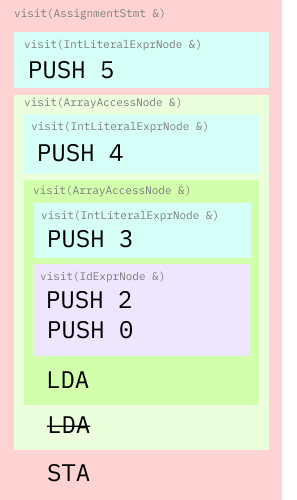
\includegraphics[width=0.35\textwidth]{lvalue_example}
\end{center}

where we have assumed (arbitrarily) that the \verb|arr| variable gets allocated to index \verb|2| in the current frame.

In the PixAR VM, the frame slot allocated to an array contains a pointer to its head. Multidimensional arrays are arrays containing pointers to the heads of other arrays. Hence, the first \verb|LDA| instruction effectively pushes a \textbf{pointer} to \verb|arr[3]| onto the work stack, which is the array which we want to store to.

If an \verb|ArrayAccessNode| is used as an rvalue, a second \verb|LDA| would load the required element from the multidimensional array. In this case, however, we remove this second \verb|LDA|, and replace it with an \verb|STA| instruction, effectively storing $5$ to the $4\textsuperscript{th}$ location of the array at the top of the working stack, which is \verb|arr[3]|.

\subsubsection{Linearization of the produced code}~\label{code-linearization}

While translating control flow statements, it is often the case that a jump instruction needs to be issued which redirects control flow to the beginning of another \verb|BasicBlock|. This can be implemented by pushing a PC-relative offset onto the work stack, and then calling one of the jump instructions.

However, there are scenarios where we do not know the offset when we need to issue the jump instruction. For example, consider the translation of an \verb|IfElseStmt|. The jump instruction needs to be issued after visiting the branch condition expression, but before visiting the if/else body. Hence we do not know ``how far forward'' we need to jump if the branch condition is not met.

To solve this problem, \verb|PUSH| instructions with relative offsets are not issued by the code generator at all. Instead a \verb|PUSH| instruction is issued with the corresponding data field set to point to the \verb|BasicBlock| that we want to jump to.

After \verb|CodeGenerator| has finished visiting all nodes in the AST, a \verb|linearizeCode()| function can be called on the \verb|PixIRCode| generated.

In one pass of the generated program, this function builds a \verb|std::map| which maps \verb|BasicBlock| pointers to the PC offset of their first instruction in the overall program.

In a separate pass, the function then uses the built map to convert \verb|BasicBlock| pointers in any \verb|PixIRInstruction|s to the corresponding PC offset.

This scheme is also advantageous for optimization passes which process the generated code, as instructions within a basic block can be transformed, and entire basic blocks or functions can be removed before linearization without invalidating any computed PC offsets.

In order to keep code generation simple, \verb|CodeGenerator| may generate some empty blocks. \verb|linearizeCode| has a final pass over the generated code where it removes these empty blocks. Note that this is safe to do after linearization, because an empty block has the same PC offset as its immediate successor.

\subsection{Optimization passes}

The implemented compiler includes three optimization passes which may improve the quality of the code produced. These passes can be enabled individually, and will be described below.

\subsubsection{Loop rotation}

The loop rotation optimization can be enabled using the \verb|-frotate-loops| flag.

It is an optimization which changes the code generated for \verb|ForStmt| and \verb|WhileStmt| nodes in such a way that only one jump instruction has to be executed per iteration of the loop.

In the regular translation of a loop, code for the loop's condition check is placed in a basic block before the body of the loop. This basic block (called the loop head) checks the condition, and jumps to the basic block immediately succeeding the loop body if the condition is not met. The last instruction in the last block of the loop body unconditionally jumps to the beginning of the loop head.

While this gives the required semantic behaviour, there are two jump instructions per iteration of the loop. For a tight loop\footnote{A tight loop is one which has a body consisting of a single basic block with only a few instructions.} the extra jump instruction may pose a significant overhead on execution.

Loop rotation duplicates the code for the condition check, and adds it to the last block in the loop body. A jump is also added which redirects control flow to the beginning of the loop body if the loop condition is met. In this way, a single iteration of the loop will only execute a single jump. Note that the loop head must be kept in place in order to handle the case where the loop condition fails immediately, since otherwise the loop body will always execute at least once. This means that the overall code size of the generated program will be larger, with this being the trade-off made for speed up.

Figure~\ref{fig:loop-rotation} shows control flow graphs for rotated and unrotated versions of a \verb|while| loop.

\begin{figure}
  \centering
  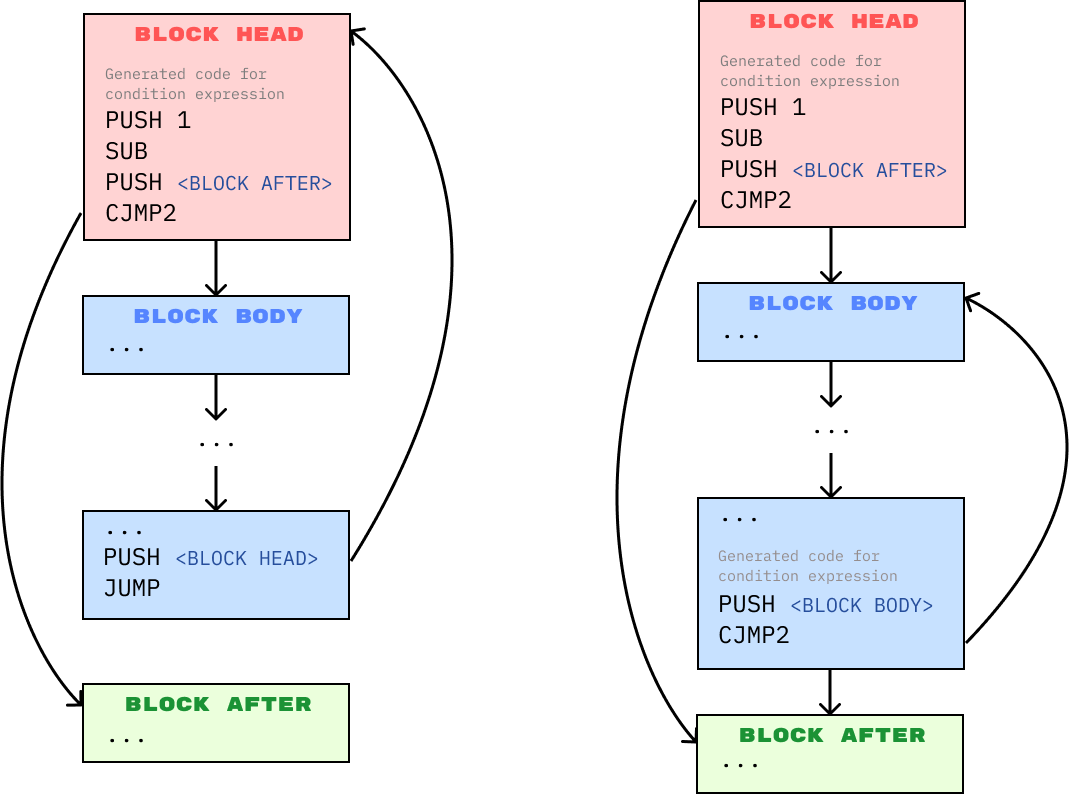
\includegraphics[width=0.8\textwidth]{loop_rotation}
  \caption{Control flow graphs for rotated (right) and unrotated (left) translations of a while statement. The rotated version contains only one jump instruction per iteration of the loop.}~\label{fig:loop-rotation}
\end{figure}

In the implementation, loop rotation is enabled/disabled for an entire program using a \verb|boolean| option in the \verb|CodeGenerator|. The \verb|visit()| methods for \verb|ForStmt| and \verb|WhileStmt| check this field, and generate code accordingly.

\subsubsection{Dead code elimination}

Dead code elimination can be enabled using the \verb|-felim-dead-code| flag, and transforms a \verb|PixIRCode| instance generated by \verb|CodeGenerator| by removing unreachable code in a basic block, as well as dead functions.

Code in a basic block is deemed unreachable if it appears after a \verb|RET| (return) instruction. In this case, the instructions can be removed safely from the basic block. This transformation is carried out in a function called \verb|eliminateDeadCodeAfterReturn|.

It is important that this pass is performed before the code linearization described in Section~\ref{code-linearization}, as removing instructions from a basic block is likely to change PC relative offsets to the start of basic blocks following the modified block.

The other transformation performed by dead code elimination is the removal of code for dead functions. A function is considered dead if it is unreachable from the main function.

In order to remove dead functions, we first use an instance of the worklist algorithm\cite{nielson2004} to find reachable functions. Pseudo code for this algorithm is shown in Algorithm~\ref{alg:reachable-worklist}.

\begin{algorithm}
   \caption{Pseudocode for the worklist algorithm used to find reachable functions.}~\label{alg:reachable-worklist}

   \KwData{
      \begin{itemize}
         \item $workList$ is a list of \Verb|PixIRFunction|s.
        \item $reachable$ is the result: A set containing the names of reachable functions.
        \item $mainFunc$ is a pointer to the \Verb|PixIRFunction| representing the main function.
      \end{itemize}}
    $workList \gets [mainFunc]$;\\
    \While{$\mathbf{length}(workList) > 0$}{
      $workListTail \gets \mathbf{pop}(workList)$;\\
      \For{$func \in \mathbf{calleesOf}(workListTail)$}{
        \If{$\mathbf{name}(func) \notin reachable$}{
          $\mathbf{insert}(reachable, \mathbf{name}(func))$;\\
          $\mathbf{push}(workList, func)$;
        }
      }
    }
\end{algorithm}

Essentially, we keep a \verb|std::vector| of pointers to \verb|PixIRFunction| instances (our worklist) which starts out with just the main function. While our worklist is non empty, we find callees of each \verb|PixIRFunction| in our worklist, add the ones we have never processed before to the worklist, and remove the processed worklist item, placing it in an \verb|std::unordered_set| which will hold all reachable functions. The worklist algorithm is encapsulated in the \verb|findReachable()| method of a class called \verb|DeadFunctionEliminator|, whose constructor takes a reference to \verb|PixIRCode| to be transformed.

Callees of a function are found by looking for \verb|PUSH| instructions in the function body where the push operand starts with a ``\verb|.|'' character, and then extracting the function name from this operand.

In order to add the corresponding \verb|PixIRFunction| to the worklist, we need a fast way of mapping function names to their \verb|PixIRFunction|. A \verb|std::unordered_map| field in \verb|DeadFunctionEliminator| is used for this purpose. During construction of an instance of this class, a single pass is performed over the \verb|PixIRCode| to be transformed, adding the mapping for each \verb|PixIRFunction| in the code to this map field.

The \verb|eliminate()| method of \verb|DeadFunctionEliminator| first calls \verb|findReachable()| to obtain a set of the names of all reachable functions. It then iterates over the code to be transformed, removing every \verb|PixIRFunction| whose name is not in this set.

\subsubsection{Peephole optimization}

The peephole optimizer transforms small runs of instructions within a single basic block. This may lead to optimization because there are situations where the \verb|CodeGenerator| may generate bad code due to locality (each \verb|visit()| method views a very small fragment of the AST).

One example of this occurs when translating an expression such as \verb|1 + x|. The ideal translation pushes the value of \verb|x| onto the work stack, uses the \verb|INC| instruction to increment the top of the stack, and then stores the value back to \verb|x|.

However, there is no clean way\footnote{\verb|dynamic_cast| could be used to check the specific type of an \verb|ExprNode| operand in the \verb|visit()| method for \verb|BinaryExprNode|. This is considered bad practice, however, and would greatly increase complexity of the code generator.} for the \verb|CodeGenerator| to know that one of the operands is an \verb|IntLiteralExprNode| with a value of $1$. Therefore, code based on the more generic \verb|ADD| instruction will be generated. The peephole optimizer can detect this situation in the generated bytecode, and transform it into code using \verb|INC|.

The peephole optimizer implemented is not very powerful, and is based on detecting exact matches for small runs of instructions, and replacing them with another run.

Small runs of instructions are represented by a type called \verb|CodePeephole|, which is an alias for a \verb|std::list| of \verb|PixIRInstruction|s.

A run of instructions intended to be matched is encapsulated in a class called \verb|PixIRPattern|. Aside from a \verb|CodePeephole| field containing the instructions to be matched, this class also has \verb|match| and \verb|match_and_replace| methods, which can check for matching runs of instructions and replace them with a given substitute.

The \verb|match()| method takes an iterator range, and checks whether the initial segment of this range matches the pattern field. A boolean is returned to indicate success or failure.

The \verb|match_and_replace()| method takes an iterator range, the \verb|std::list| this range is taken from (which will be the list of instructions in the basic block being optimized), as well as a \verb|CodePeephole| containing the run of instructions that will be substituted for a match. The \verb|match()| method is used to check whether the initial segment of the iterator range contains the required pattern. If this is the case, the \verb|erase()|/\verb|insert()| methods of \verb|std::list| are used to replace the matched run of instructions with the substitute.

A global, constant \verb|patterns| variable maps \verb|PixIRPattern|s to the corresponding substitute run. For example, the \verb|PixIRPattern| containing the run of instructions \verb|PUSH 1; ADD| is mapped to the substitute \verb|INC|.

The \verb|peepholeOptimize()| function puts everything together: it takes a \verb|PixIRCode| instance and iterates over each of its basic blocks' list of instructions, calling \verb|match_and_replace()| for every pattern in \verb|patterns| at each location in the list.

This peephole optimizer has some obvious limitations. The largest shortcoming stems from the fact that it can only match exact runs of instructions. So for example any program of the form $e$\verb| + 1| where $e$ is an arbitrary expression will not be optimized to use \verb|INC|, because there is no way to match the instructions for the arbitrary expression in the generated code.

\newpage

\bibliographystyle{ieeetr}
\bibliography{references}

\end{document}
